\documentclass[final]{beamer}
\usepackage{grffile}
\mode<presentation>
\usetheme{le2i}
\usepackage[english]{babel}
%\usepackage[latin1]{inputenc}
\usepackage{amsmath,amsthm, amssymb, latexsym}
\usepackage{multirow}
\usepackage{algorithm}
\usepackage{algpseudocode}
\usepackage{latexsym}
\usepackage{xcolor}
\usepackage{epsf,graphicx,subfig}
\usepackage{epstopdf}
\usepackage{subfig}	
%% In order to draw some graphs
\usepackage{tikz,xifthen}
\usetikzlibrary{decorations.pathmorphing}
\usetikzlibrary{fit}
\usetikzlibrary{backgrounds}
\usetikzlibrary{shapes,arrows,shadows}
\usetikzlibrary{calc,decorations.pathreplacing,decorations.markings,positioning}
\usetikzlibrary{snakes,decorations.text,shapes,patterns}

\boldmath
\usepackage[orientation=landscape,size=a0,scale=1.4,debug]{beamerposter}
% change list indention level
% \setdefaultleftmargin{3em}{}{}{}{}{}


\usepackage{array,booktabs,tabularx}
\newcolumntype{Z}{>{\centering\arraybackslash}X} % centered tabularx columns
\newcommand{\pphantom}{\textcolor{ta3aluminium}} % phantom introduces a vertical space in p formatted table columns??!!

\usepackage{lipsum}

\listfiles

%%%%%%%%%%%%%%%%%%%%%%%%%%%%%%%%%%%%%%%%%%%%%%%%%%%%%%%%%%%%%%%%%%%%%%%%%%%%%%%%%%%%%%
\graphicspath{{images/}}
 
\title{\huge Your Title }
\author{Authors }
\institute[Univerist\'e de Bourgogne]{Institute and Universities }
\date[May. 26th 2015]{May. 26th 2015}

%{Le2i-UMR CNRS 6306, BP 47870, 21078 Dijon, France\\
%Computer Vision and Robotics Group, Campus Montilivi, Edifici PIV, s/n, 17071 Girona, Spain}

%%%%%%%%%%%%%%%%%%%%%%%%%%%%%%%%%%%%%%%%%%%%%%%%%%%%%%%%%%%%%%%%%%%%%%%%%%%%%%%%%%%%%%
\newlength{\columnheight}
\setlength{\columnheight}{91cm}


%%%%%%%%%%%%%%%%%%%%%%%%%%%%%%%%%%%%%%%%%%%%%%%%%%%%%%%%%%%%%%%%%%%%%%%%%%%%%%%%%%%%%%
\begin{document}
\begin{frame}
  \begin{columns}
    % ---------------------------------------------------------%
    % Set up a column 
    
    %----------------------------------------------------------%
    %             		FIRST COLUMN 						  %
	%----------------------------------------------------------%
    \begin{column}{.33\textwidth}
      \begin{beamercolorbox}[center,wd=\textwidth]{postercolumn}
        \begin{minipage}[T]{.95\textwidth}  % tweaks the width, makes a new \textwidth
          \parbox[t][\columnheight]{\textwidth}{ % must be some better way to set the the height, width and textwidth simultaneously
            % Since all columns are the same length, it is all nice and tidy.  You have to get the height empirically
            % ---------------------------------------------------------%

            % fill each column with content            
            \begin{block}{Abstract}
              \lipsum[1-2]
            \end{block}
            \begin{block}{Introduction}
              \begin{itemize}
               \item \textbf{\color{titlescolor} First point }
               \begin{itemize}
               		\item Description 
               		\item More description
               \end{itemize}  
              \end{itemize}                 
            \end{block}
            \begin{block}{Second block}
            \begin{itemize}
            	\item \textbf{\color{titlescolor}Random forest (RF) ensemble}
            	\item []
            	\item []
            	\begin{columns}
            		\begin{column}{.54\textwidth}
            		\centering{Training}\\
            			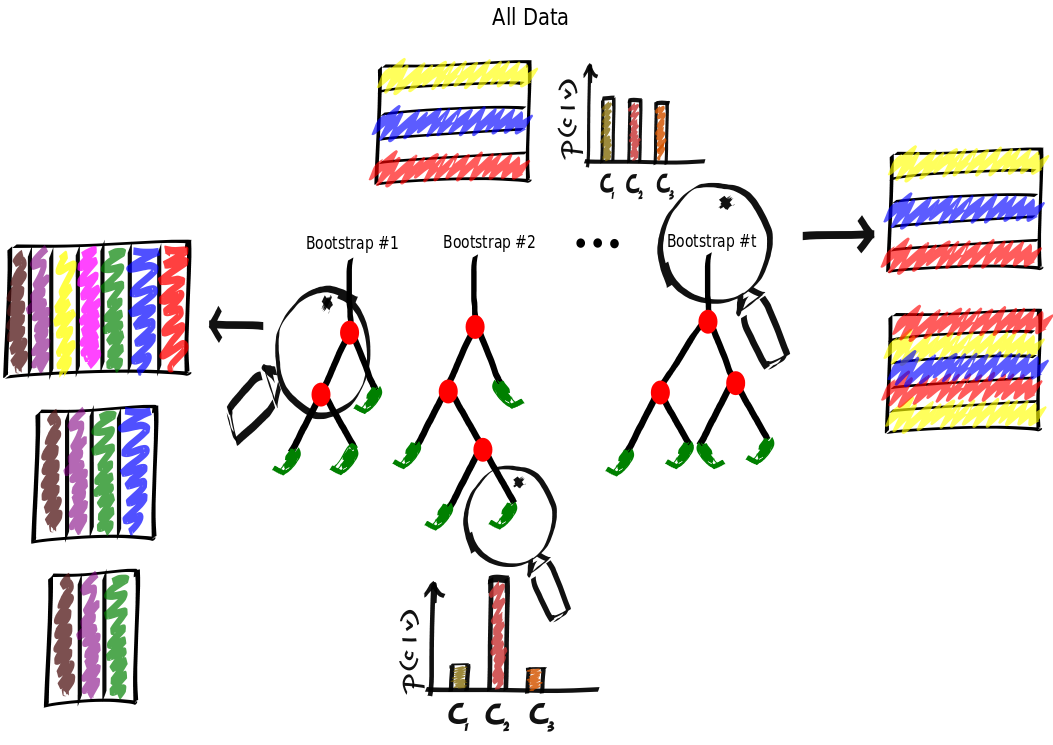
\includegraphics[width = 0.9\textwidth, height = 0.15\textheight]{images/framework/RF_train.png}
            		\end{column}
            		\begin{column}{.44\textwidth}
            		\centering{Testing}\\
            			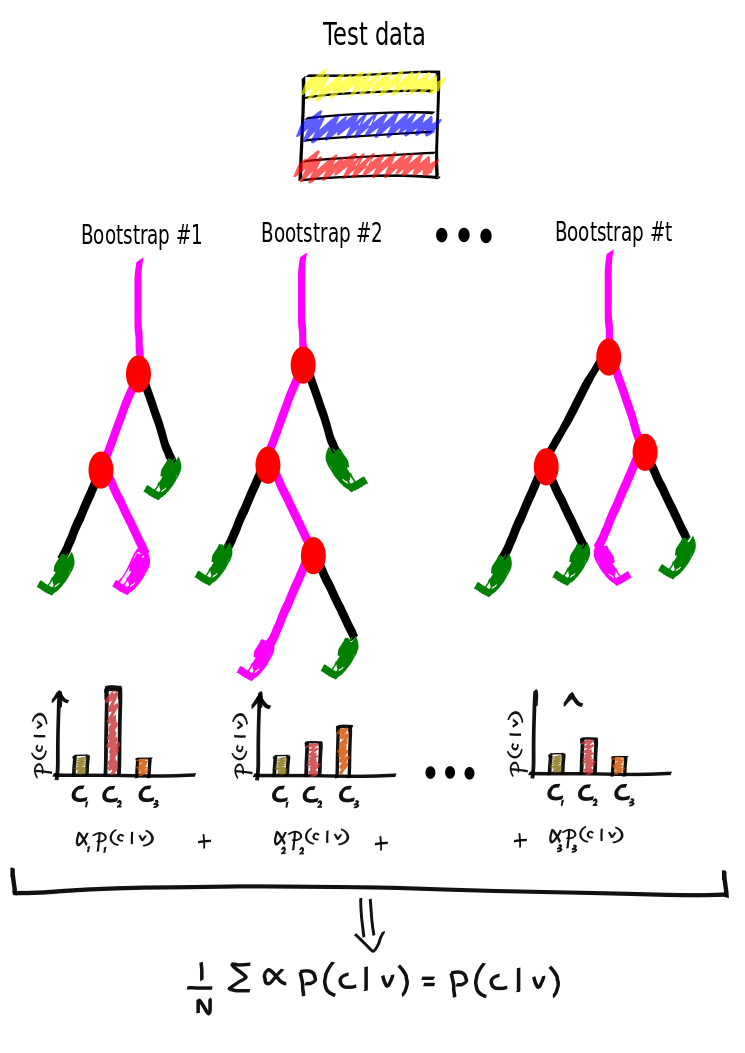
\includegraphics[width = 0.9\textwidth, height = 0.15\textheight]{images/framework/RF_test.png}
            		\end{column}
            \end{columns}
            \end{itemize}
            \end{block}          
            \vfill
         
           }
        \end{minipage}
      \end{beamercolorbox}
    \end{column}
    %----------------------------------------------------------------%
    %                      SECOND COLUMN                             % 
    %----------------------------------------------------------------%
    \begin{column}{.33\textwidth}
      \begin{beamercolorbox}[center,wd=\textwidth]{postercolumn}
        \begin{minipage}[T]{.95\textwidth}  % tweaks the width, makes a new \textwidth
          \parbox[t][\columnheight]{\textwidth}{ % must be some better way to set the the height, width and textwidth simultaneously
            % Since all columns are the same length, it is all nice and tidy.  You have to get the height empirically
            % ---------------------------------------------------------%

            % fill each column with content            
            \begin{block}{Franework}
              \lipsum[1-2]
                 \begin{equation}
                   {n! \over k!(n-k)!} = {n \choose k}
                 \end{equation}
                 \lipsum[1]\cite{barata2014color, barata2013towards, barata2013role, barata2013two, barata2014bag}
            \end{block}
            \vfill
  

         
           }
        \end{minipage}
      \end{beamercolorbox}
    \end{column}
    %----------------------------------------------------------%
    %             		Third COLUMN 						  %
	%----------------------------------------------------------%
	\begin{column}{.33\textwidth}
	\begin{beamercolorbox}[center,wd=\textwidth]{postercolumn}
        \begin{minipage}[T]{.95\textwidth}  % tweaks the width, makes a new \textwidth
          \parbox[t][\columnheight]{\textwidth}{ % must be some better way to set the the height, width and textwidth simultaneously
            % Since all columns are the same length, it is all nice and tidy.  You have to get the height empirically
            \begin{block}{Fourth block}
            	 \begin{itemize}
            		\item \textbf{\color{titlescolor} title }
            		\begin{itemize}
            		 \item {\color{orounam} Description }
            		\end{itemize}
            	 \end{itemize}
                 \lipsum[1-2]
            \end{block}
            \begin{block}{References}
              \bibliography{refs2}
 			  \bibliographystyle{unsrtnat}
            \end{block}
            }
        \end{minipage}
    \end{beamercolorbox}    
	\end{column}
    % ---------------------------------------------------------%
    % end the column
  \end{columns}
  \vskip1ex

  %\tiny\hfill\textcolor{ta2gray}{Created with \LaTeX \texttt{beamerposter}  \url{http://www-i6.informatik.rwth-aachen.de/~dreuw/latexbeamerposter.php}}
  \tiny\hfill{Created with \LaTeX \texttt{beamerposter}  \url{http://www-i6.informatik.rwth-aachen.de/~dreuw/latexbeamerposter.php} \hskip1em}
\end{frame}
\end{document}


%%%%%%%%%%%%%%%%%%%%%%%%%%%%%%%%%%%%%%%%%%%%%%%%%%%%%%%%%%%%%%%%%%%%%%%%%%%%%%%%%%%%%%%%%%%%%%%%%%%%
%%% Local Variables: 
%%% mode: latex
%%% TeX-PDF-mode: t
%%% TeX-master: t
%%% End:
